%%%%%%%%%%%%%%%%%%%%%%%%%%%%%%%%%%%%%%%%%%%%
%% TABLE: DISTRIBUTION OF DEATHS BY CAUSE %%
%%%%%%%%%%%%%%%%%%%%%%%%%%%%%%%%%%%%%%%%%%%%
\begin{table}[H]
  \caption{Distribution of Deaths by Cause, Ages 25--69 (2018)}
  \label{tab:icd_causes}
  \begin{tabular}{lc}
    Cause of Death & Share of Total Deaths \\
    \hline
    Cancer&28.28\\
Heart and other diseases of the circulatory system&21.75\\
Poisoning, suicide, chronic liver disease ("deaths of despair") &11.82\\
Diseases of the respiratory system&8.00\\
Accidents and injuries (primarily falls, motor vehicles, assaults)&5.79\\
Endocrine, nutritional and metabolic diseases&5.36\\
Diseases of the nervous system&3.69\\
Cerebrovascular diseases&3.33\\
Infectious and parasitic diseases&2.72\\
Diseases of the digestive system&2.48\\
Diseases of the genitourinary system&1.95\\
Mental and behavioural disorders&1.92\\
Deaths not elsewhere classified&0.95\\
Diseases of the blood and immune disorders&0.88\\
Diseases of the musculoskeletal system and connective tissue&0.53\\
Congenital malformations, deformations and chromosomal abnormalities&0.27\\
Diseases of the skin and subcutaneous tissue&0.19\\
Pregnancy, childbirth and the puerperium&0.07\\
Diseases of the eye, ear, mastoid and adnexa&0.01\\
Certain conditions originating in the perinatal period&0.00\\

    \hline
  \end{tabular}
  \footnotesize{Note: The table shows the distribution of causes of
    death for individuals aged 25--69 in 2018. Categories are defined
    by major headings in the ICD-10 Cause-Of-Death lists. The
    categories of cancer, heart disease and deaths of despair are
    pooled across subcategories following the previous literature. See
    Appendix~\ref{sec:app_data} for additional details.}
\end{table}

%%%%%%%%%%%%%%%%%%%%%%%%%%%%%%%%%%%%%%%%%%%%%%%%%%%%%%
%% TABLE: AGE-ADJUSTED MORTALITY CHANGES, BY CAUSES %%
%%%%%%%%%%%%%%%%%%%%%%%%%%%%%%%%%%%%%%%%%%%%%%%%%%%%%%
\begin{landscape}
  \begin{table}[htbp]
    \caption{Age-Adjusted Changes in Mortality by
      Education Percentile and Cause \cnewline Ages 25--69, 1992--1994
      to 2016--2018}
    \label{tab:all_cause_all_age}
    \centering
\resizebox{\columnwidth}{!}{%
  \begin{tabular}{llcccccc}
  & & Injuries & Cancer & Heart Disease & Despair & Other & Total \\
  \hline
  \textbf{White non-Hispanic Women} & & & & & & & \\
  Education Percentile &  0--10  & (+62\%, +79\%) & (+25\%, +35\%) & (+3\%, +38\%) & (+526\%, +585\%) & (+111\%, +167\%) & (+77\%, +111\%) \\
                       & 10--45  & (+15\%, +36\%) & (-26\%, -18\%) & (-38\%, -16\%) & (+274\%, +354\%) & (+18\%, +52\%) & (-0\%, +21\%) \\
                       & 45--70  & (-29\%, +21\%) & (-48\%, -37\%) & (-59\%, -28\%) & (+64\%, +225\%) & (-26\%, +26\%) & (-39\%, -4\%) \\
                       & 70--100 & (-50\%, -34\%) & (-49\%, -47\%) & (-61\%, -55\%) & (-14\%, +42\%) & (-38\%, -28\%) & (-48\%, -39\%) \\

  \hline
  \textbf{White non-Hispanic Men} & & & & & & & \\
  Education Percentile &  0--10  & (+32\%, +47\%) & (+17\%, +27\%) & (+1\%, +13\%) & (+241\%, +267\%) & (+70\%, +102\%) & (+50\%, +68\%) \\
                       & 10--45  & (+2\%, +16\%) & (-30\%, -24\%) & (-38\%, -31\%) & (+156\%, +186\%) & (+3\%, +16\%) & (-6\%, +5\%) \\
                       & 45--70  & (-22\%, +15\%) & (-52\%, -42\%) & (-58\%, -45\%) & (+78\%, +148\%) & (-36\%, -14\%) & (-40\%, -18\%) \\
                       & 70--100 & (-44\%, -35\%) & (-55\%, -52\%) & (-63\%, -59\%) & (+17\%, +39\%) & (-54\%, -48\%) & (-52\%, -45\%) \\

  \hline
  \textbf{Black non-Hispanic Women} & & & & & & & \\
  Education Percentile &  0--10  & (+11\%, +19\%) & (-9\%, -6\%) & (-16\%, -11\%) & (+152\%, +168\%) & (+23\%, +32\%) & (+11\%, +17\%) \\
                       & 10--45  & (-33\%, -24\%) & (-31\%, -28\%) & (-42\%, -37\%) & (+44\%, +65\%) & (-21\%, -12\%) & (-28\%, -21\%) \\
                       & 45--70  & (-49\%, -25\%) & (-45\%, -40\%) & (-60\%, -49\%) & (-8\%, +48\%) & (-38\%, -20\%) & (-47\%, -33\%) \\
                       & 70--100 & (-60\%, -51\%) & (-49\%, -48\%) & (-67\%, -64\%) & (-41\%, -22\%) & (-51\%, -45\%) & (-55\%, -51\%) \\

  \hline
  \textbf{Black non-Hispanic Men} & & & & & & & \\
  Education Percentile &  0--10  & (+28\%, +39\%) & (-22\%, -19\%) & (-12\%, -10\%) & (+109\%, +118\%) & (-8\%, -4\%) & (-0\%, +3\%) \\
                       & 10--45  & (-18\%, -8\%) & (-46\%, -44\%) & (-37\%, -33\%) & (+30\%, +40\%) & (-36\%, -32\%) & (-33\%, -29\%) \\
                       & 45--70  & (-48\%, -21\%) & (-63\%, -57\%) & (-56\%, -49\%) & (-8\%, +22\%) & (-54\%, -45\%) & (-54\%, -44\%) \\
                       & 70--100 & (-69\%, -63\%) & (-68\%, -66\%) & (-66\%, -63\%) & (-45\%, -34\%) & (-69\%, -66\%) & (-67\%, -64\%) \\
\hline & & & & & & & \\
\end{tabular}
}

  \end{table}
  \footnotesize{ Note: The table shows age-adjusted percentage change
    in mortality from 1992--1994 to 2016--2018 for individuals aged 25
    to 69, by race, gender and education percentile bin. Each table
    entry shows the upper and lower bound on the percentage change in
    mortality over the sample period for the given cause and
    population subgroup. Ages are adjusted with a standardized
    U.S. population distribution, which holds constant that age
    distribution of the population across all years. Education
    percentile bins approximately describe the 2003 distribution of
    education across four categories: high schools dropouts
    (percentiles 0--10), high school graduates (10--45), some college
    (45--70) and B.A. or higher (70--100).}
\end{landscape}

%%%%%%%%%%%%%%%%%%%%%%%%%%%%%%%%%%%%%%%%%%%%%%%%%
%% FIGURE: BOUND ESTIMATES AND NAIVE ESTIMATES %%
%%%%%%%%%%%%%%%%%%%%%%%%%%%%%%%%%%%%%%%%%%%%%%%%%
\begin{figure}[H]
  \floatpagestyle{empty}
  \caption{Bounds on Constant Percentile Mortality Change and Naive
    Point Estimates \cnewline Age-Adjusted Populations, 1992--1994 to 2016--2018}
  \label{fig:bias}
  \begin{center}
    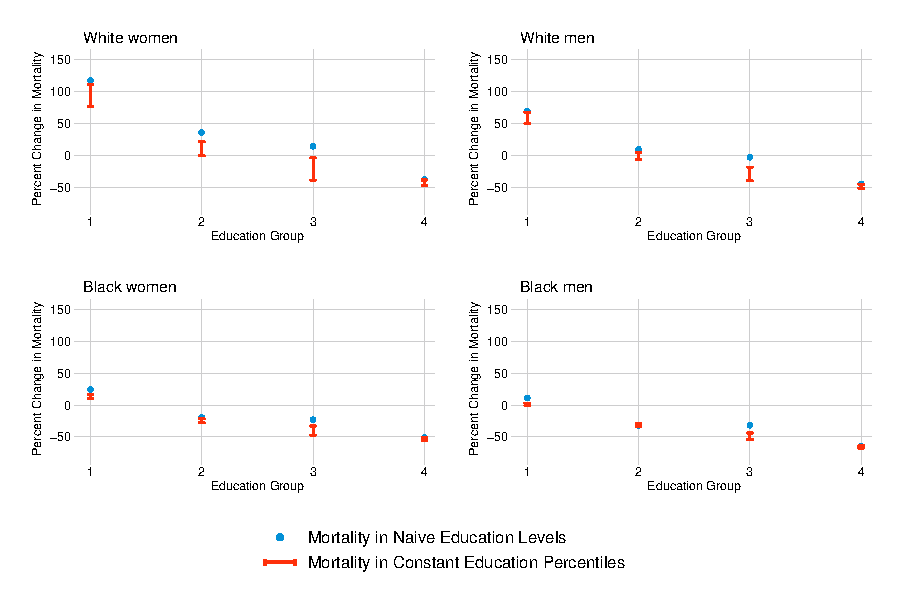
\includegraphics[scale=1.1]{\mortalitypath/std_mort_perc_total}
  \end{center}
  \footnotesize{Note: ``White'' refers to non-Hispanic white and
    ``Black'' to non-Hispanic black. The line segments in the graph
    show bounds on age-adjusted mortality change from 1992--1994 to
    2016--2018 for a standardized population, as in
    Table~\ref{tab:mort_changes}. The four education groups represent
    education percentiles (i) 0--10; (ii) 10--45; (iii) 45--70; and (iv) 70--100.
    The points in the graph show naive estimates of mortality rates at
    fixed education \textit{levels}; the four education levels for the
    points represent (i) high school dropouts; (ii) high school
    completers; (iii) some college; and (iv) a B.A. or higher.}
\end{figure}

%%%%%%%%%%%%%%%%%%%%%%%%%%%%%%%%%%%%%%%%%%%%%%%%%%%%%%%%%%%%%%%%%%%%%%%%
%% FIGURE: BOUND ESTIMATES AND NAIVE ESTIMATES -- ALL RACE-SEX GROUPS %%
%%%%%%%%%%%%%%%%%%%%%%%%%%%%%%%%%%%%%%%%%%%%%%%%%%%%%%%%%%%%%%%%%%%%%%%%
\begin{landscape}
\begin{figure}[H]
  \floatpagestyle{empty}
  \caption{Bounds on Constant Percentile Mortality Change and Naive
    Point Estimates: \cnewline 50--54-year-olds, 1992--1994 to 2016--2018}
  \label{fig:bias_more}
  \begin{center}
    \begin{tabular}{cc}
      \multicolumn{2}{c}{\textul{White Women}} \\
      Dropouts vs. p0--p17 & High School vs. p17--p60 \\
      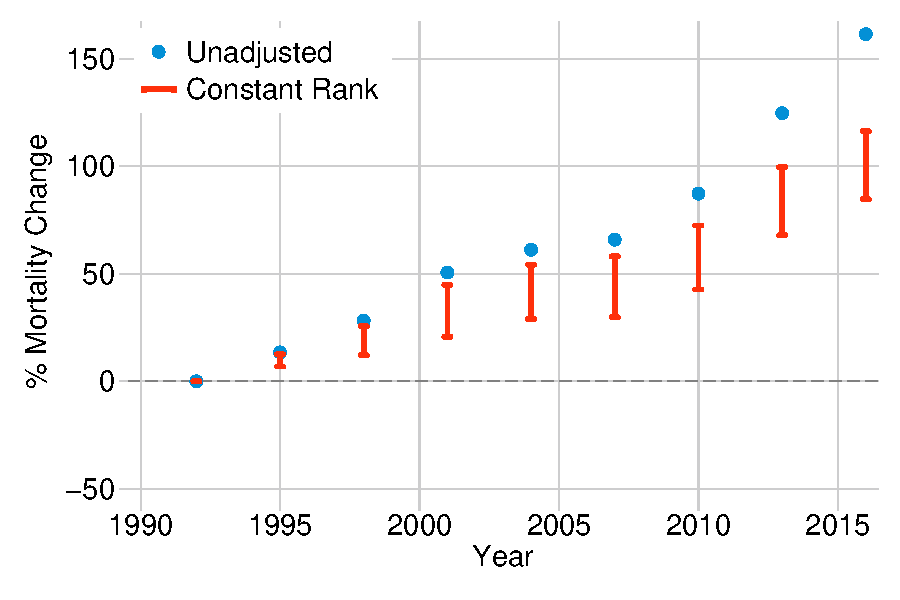
\includegraphics[scale=0.6]{\mortalitypath/naive-1-women-50-t-1} &
      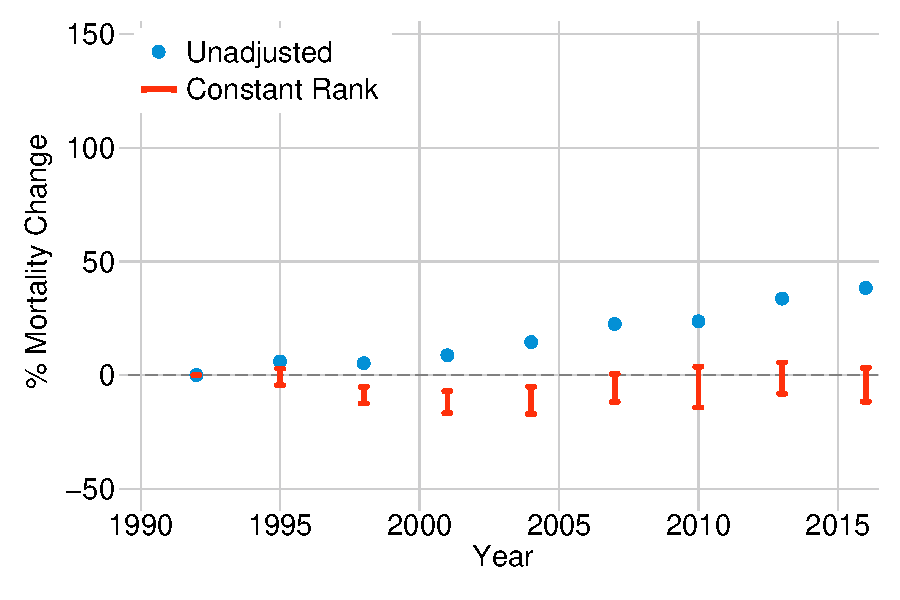
\includegraphics[scale=0.6]{\mortalitypath/naive-1-women-50-t-2} \\

      \multicolumn{2}{c}{\textul{White Men}} \\
      Dropouts vs. p0--p17 & High School vs. p17--p52 \\
      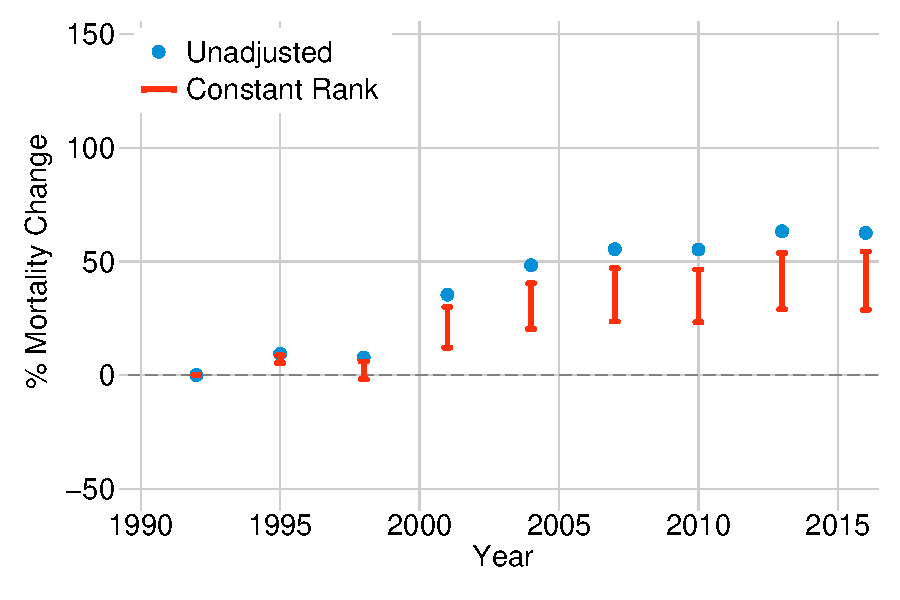
\includegraphics[scale=0.6]{\mortalitypath/naive-1-men-50-t-1} &
      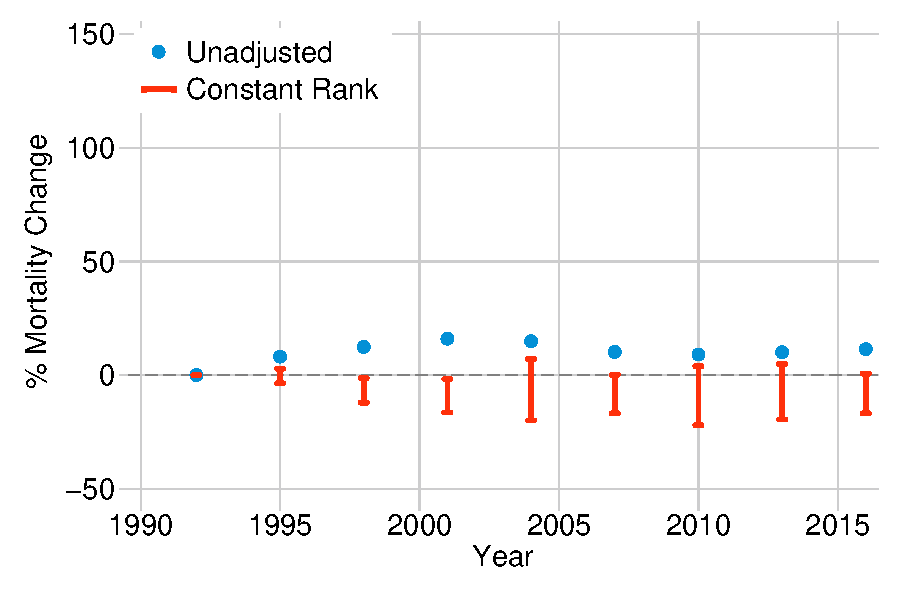
\includegraphics[scale=0.6]{\mortalitypath/naive-1-men-50-t-2} \\
      
    \end{tabular}
  \end{center}
  \end{figure}
\begin{figure}[H]\ContinuedFloat
  \begin{center}
    \begin{tabular}{cc}
      
      \multicolumn{2}{c}{\textul{Black Women}} \\
      Dropouts vs. p0--p17 & High School vs. p17--p60 \\
      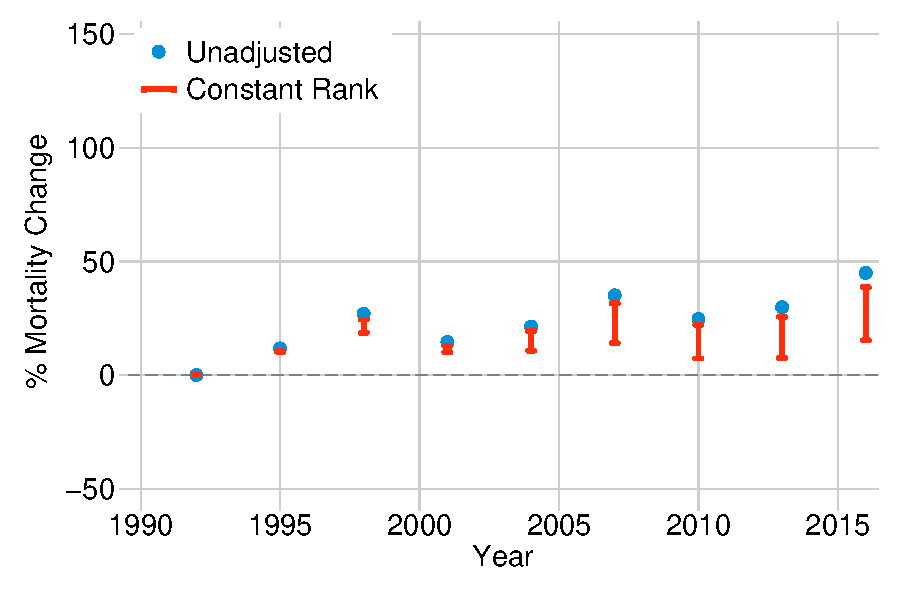
\includegraphics[scale=0.6]{\mortalitypath/naive-2-women-50-t-1} &
      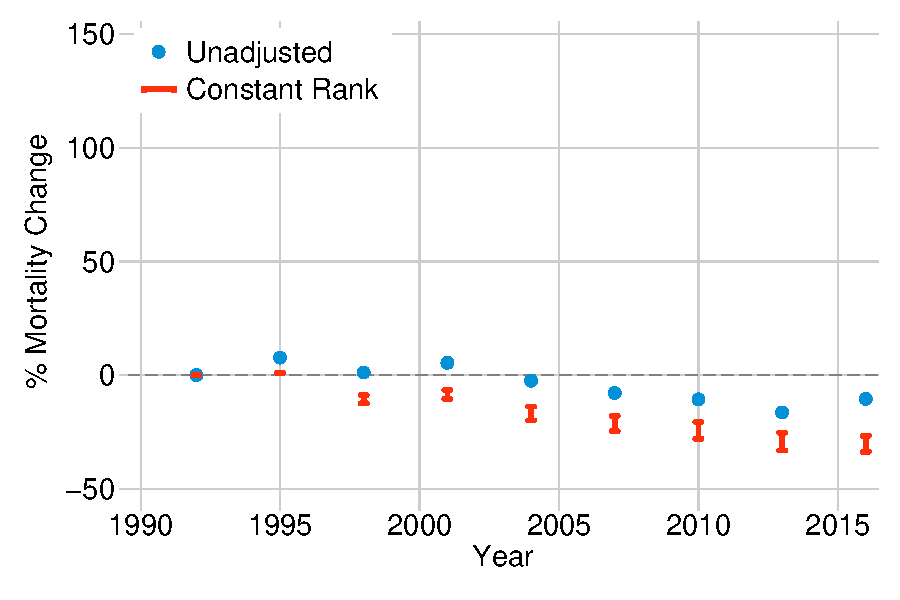
\includegraphics[scale=0.6]{\mortalitypath/naive-2-women-50-t-2} \\

      \multicolumn{2}{c}{\textul{Black Men}} \\
      Dropouts vs. p0--p17 & High School vs. p17--p52 \\
      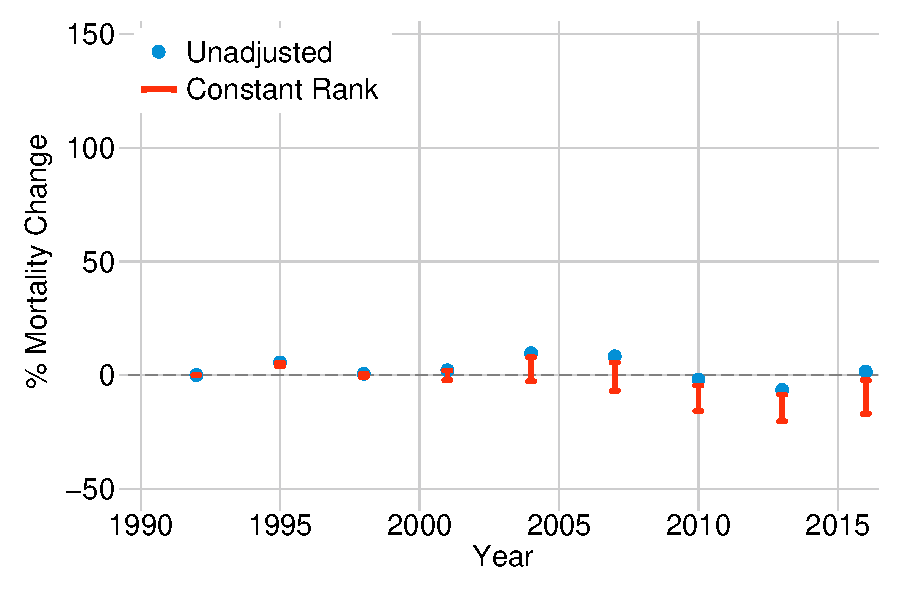
\includegraphics[scale=0.6]{\mortalitypath/naive-2-men-50-t-1} &
      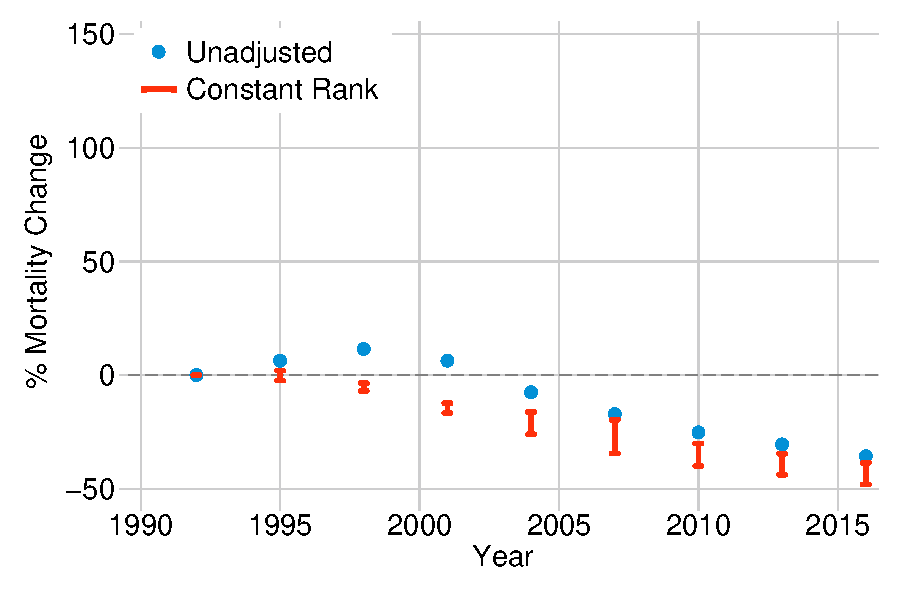
\includegraphics[scale=0.6]{\mortalitypath/naive-2-men-50-t-2} \\

    \end{tabular}
    
  \end{center}
  \footnotesize{Note: ``White'' refers to non-Hispanic white and ``Black'' to non-Hispanic black. The line segments in the graph show bounds on age-adjusted mortality change from 1992--1994 to 2016--2018 for 50-year-olds, separately by race and gender. The four education groups represent education percentiles (i) 0--10; (ii) 10--45; (iii) 45--70; and (iv) 70--100.  The points in the graph show naive estimates of mortality rates at fixed education \textit{levels}; the four education levels for the points represent (i) high school dropouts; (ii) high school completers; (iii) some college; and (iv) a B.A. or higher.}
\end{figure}
\end{landscape}

